\documentclass[../main.tex]{subfiles}
\begin{document}

    \subfile{010-010-intro}

    \section{History of Data Science}
        \label{se:intro-ds-history}

        Statistics, data science, and computational programming education
        have co-evolved in the last half-century.
        While the term ``data science'' started to grow in popularity in 2014
        (according to Google Trends),
        the ideas behind data science began in the 1960s, if not earlier,
        and the computing technology behind all the computation needed
        to create insights evolved in tandem.

        \subfile{010-020-ds_history}
        \subfile{010-030-r_history}
        \subfile{010-040-python_history}
        \subfile{010-045-emerging_technologies}
        \subfile{010-050-swc_history}

    \section{Data Science Education and Pedagogy Research}
        \label{se:intro-ds-edu-ped}

        Computing and statistics education have both created their own sets of
        higher education curriculum guidelines.
        Many of these concepts have made their way down from higher education to K-12,
        suggesting the top-down need for learning data science skills.

        \subfile{010-060-computing_education}
        \subfile{010-080-statistics_education}
        \subfile{010-070-data_science_education}

    \section{Learner Personas and Pedagogical Backed Strategies for Creating Accessible Content in Data Science}
        \label{se:intro-personas}

        \subfile{010-110-personas}

    \section{Best Practices in Teaching Data Science}
        \label{se:intro-teaching-best-practices-ds}

        \subfile{010-120-best_practices}

    \section{The Need for Pedagogically-Backed Data Science Curriculum in Medicine}
        \label{se:intro-ds-edu-gaps}

        \subfile{010-130-domain-ds-materials}

    \section{Building a Community (of Practice)}

        This dissertation does not explicitly explore the process of online community building,
        but this is an important idea to keep in mind when creating educational materials,
        as connecting with other educators to form a community of practice
        where (typically geographically co-located) people with a common set of goals, interests, and concerns
        can learn from one another
        \cite{wilson2019teaching}.
        Organizations like The Carpentries can provide online teaching communities of practice
        where other instructors can learn from one another around
        builing the pedagogical content knowledge for teaching, not just around data science
        \cite{CarpentriesHowWe, shulmanThoseWhoUnderstand1986}.

        Community building is a slow process, and there are four (4) main components on building and sustaining a community.
        The first step is onboarding and recruiting new members.
        A Code of Conduct should be prominent during this phase of community building and ensure members are in a safe environment.
        Onboarding should also include resources to bring new members up to date on current community events.
        The second step is around retention.
        Community members should have some sense of agency and be able to contribute to the group,
        and these contributions should be acknowledged.
        As communities grow, eventually a governance model will need to be created to help
        provide top-down guidance for major decisions.
        These governance models do not need to be strictly hierarchical,
        and can adapt with the size of the community.
        Finally, retention and onboarding is a never-ending process.
        Healthy communities plan for the efflux of members by onboarding more members and helping to retain them.

        This dissertation primarily focuses on the learners, and finding ways to improve their learning.
        Teaching is an art and skill on its own
        \cite{greenBuildingBetterTeacher2014, wilson2019teaching}.
        Knowing what needs to be taught (content knowledge),
        how the materials are taught (pedagogical content knowledge), and
        why topics are taught in context (curricular knowledge)
        are all aspects of teaching knowledge that instructors can benefit from joining a teaching
        community of practice
        \cite{shulmanThoseWhoUnderstand1986, greenBuildingBetterTeacher2014, wilson2019teaching}.

    \section{Ethics}

    One of the more prominent data science workflow figures comes from the R4DS book reproducted in
    Figure \ref{fig:r4ds-data_science} \cite{wickhamR4ds}.
    Many of these figures that discuss the data science workflow miss the opporunity to discuss how
    the data products that come out of data science and the decisions that come from communicating findings,
    affects the world ((e.g., Figures \ref{fig:conway-venn} and \ref{fig:gaisek-12})).

    \begin{figure}[!hbtp]
        \centering
        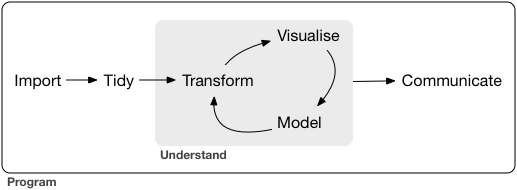
\includegraphics[scale=0.5]{figs/050-intro/r4ds-data-science}
        \caption[R4DS: Data Science Workflow]{
        Reproduction of the data science workflow from R4DS \cite{wickhamR4ds}.
        }
        \label{fig:r4ds-data_science}
    \end{figure}

    In practice, there many cycles within the data science process; it is typically not a linear process from
    data collection to communicating results for a decision.
    Each of the steps within the data science process has the potential for errors and biases.
    Among one of the cycles within the data science process is the cycle between how decisions made from the data science process affect the world
    (Figure \ref{fig:data_science_consequences}).
    Many of the data ethics issues can be accounted for by being more mindful of how data science have real-world consequences.

    \begin{figure}[!hbtp]
        \centering
        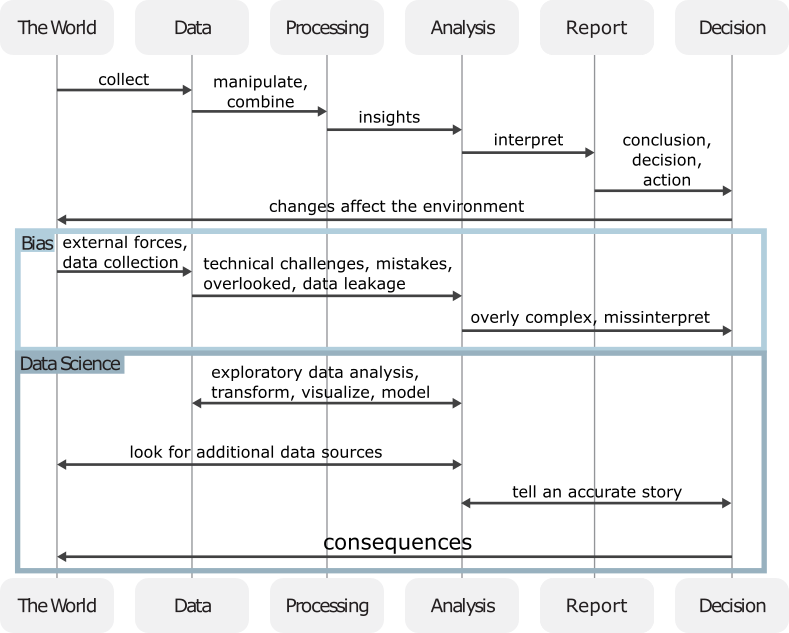
\includegraphics[scale=0.5]{figs/050-intro/data_science_figure}
        \caption[Data Science and It's Consequences]{
        The data science process showing the same cycles as previous data science figures.
        This figure puts an emphasis on how the decisions from data products have real-world consequences that feedback into
        the data science process \cite{Chen2020}.
        }
        \label{fig:data_science_consequences}
    \end{figure}

    Reproducibility failures (Figure \ref{fig:data_science_consequences} adapted
    from \cite{ostblomOpinionatedPracticesTeaching2021}) are one way where data
    science can have consequences in the real-world
    \cite{aboumatarNoticeRetractionAboumatar2019, ExcelWhyUsing2020,
    ostblomOpinionatedPracticesTeaching2021,
    wallensteenRetractionNoticeEvaluation2018,
    whitehouseRetractionNoteComplex2021, zeebergMistakenIdentifiersGene2004,
    ziemannGeneNameErrors2016}.

    \begin{figure}[!hbtp]
        \centering
        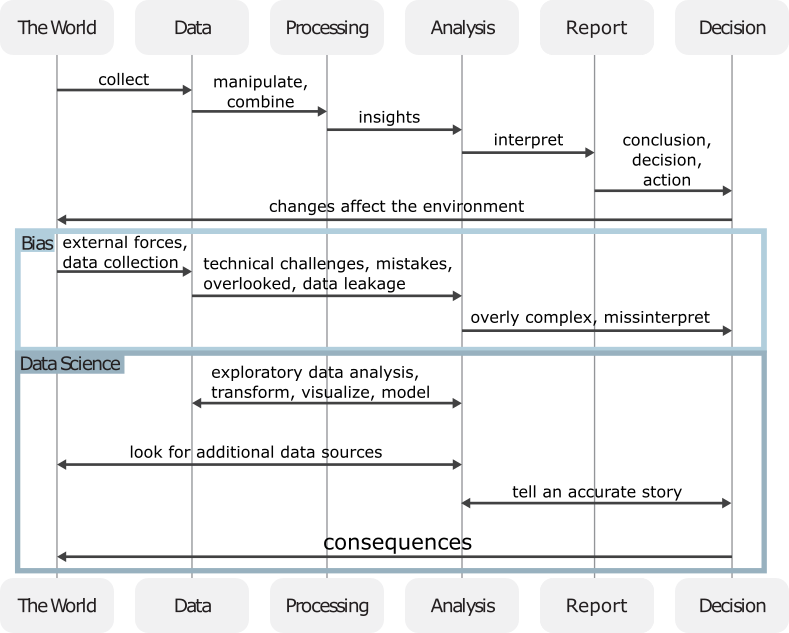
\includegraphics[scale=0.5]{figs/050-intro/data_science_figure}
        \caption[Data Science and It's Consequences]{
        The data science process showing the same cycles as previous data science figures.
        This figure puts an emphasis on how the decisions from data products have real-world consequences that feedback into
        the data science process \cite{Chen2020}.
        }
        \label{fig:data_science_consequences}
    \end{figure}

    Aside from technical issues that can cause adverse real-world impacts, data
    science and healthcare have numerous ethical questions as well
    \cite{gerkeEthicalLegalChallenges2020, peekThirtyYearsArtificial2015,
    phannonstanford.eduResearchersSayUse, rigbyEthicalDimensionsUsing2019,
    wetsmanWHOOutlinesPrinciples2021}.
    In healthcare, there are primiarly 4 ethical challenges:
    (1) informed consent to use,
    (2) safety and transparency,
    (3) algorithmic fairness and biases, and
    (4) data privacy
    \cite{gerkeEthicalLegalChallenges2020}.
    While data science has the potential to revolutionalize medical research,
    a high level of scruteny must be employed to adequately and safely work with
    data that will have real impacts on patients.


    %


    % \cite{ostblomOpinionatedPracticesTeaching2021}

    % https://journalofethics.ama-assn.org/article/ethical-dimensions-using-artificial-intelligence-health-care/2019-02

    % https://www.sciencedirect.com/science/article/pii/S0933365715000871?via%3Dihub

    % https://www.ncbi.nlm.nih.gov/pmc/articles/PMC7332220/

    % https://med.stanford.edu/news/all-news/2018/03/researchers-say-use-of-ai-in-medicine-raises-ethical-questions.html

    % https://www.theverge.com/2021/6/30/22557119/who-ethics-ai-healthcare


\end{document}
